%%%%%%%%%%%%%%%%%%%%%%%%%%%%%%%%%%%%%%%%%%%%%%%%%%%%%%%%%%%%%%%%%%%%%%%%%%%
%
% Generic template for TFC/TFM/TFG/Tesis
%
% $Id: resultados.tex,v 1.7 2016/03/31 10:44:23 macias Exp $
%
% By:
%  + Javier Macías-Guarasa.
%    Departamento de Electrónica
%    Universidad de Alcalá
%  + Roberto Barra-Chicote.
%    Departamento de Ingeniería Electrónica
%    Universidad Politécnica de Madrid
% 
% Based on original sources by Roberto Barra, Manuel Ocaña, Jesús Nuevo, Pedro Revenga, Fernando Herránz and Noelia Hernández. Thanks a lot to all of them, and to the many anonymous contributors found (thanks to google) that provided help in setting all this up.
%
% See also the additionalContributors.txt file to check the name of additional contributors to this work.
%
% If you think you can add pieces of relevant/useful examples, improvements, please contact us at (macias@depeca.uah.es)
%
% You can freely use this template and please contribute with comments or suggestions!!!
%
%%%%%%%%%%%%%%%%%%%%%%%%%%%%%%%%%%%%%%%%%%%%%%%%%%%%%%%%%%%%%%%%%%%%%%%%%%%

\chapter{Resultados}
\label{cha:resultados}


\begin{FraseCelebre}
  \begin{Frase}
    % Si quieres ser leído más de una vez, no vaciles en borrar a menudo.
    Rem tene, verba sequentur (Si dominas el tema, las palabras vendrán solas)\footnote{Tomado de ejemplos del proyecto \texis{}.}.
  \end{Frase}
  \begin{Fuente}
    % Horacio
    Catón el Viejo
  \end{Fuente}
\end{FraseCelebre}

\section{Introducción}
\label{sec:introduccion-resultados}

En este capítulo se introducirán los resultados más relevantes del trabajo.

La estructura del capítulo es\ldots


\section{Entorno experimental}
\label{sec:entorno-experimental}

Blah, blah, blah.


\subsection{Bases de datos utilizadas}
\label{sec:bases-de-datos-1}

Blah, blah, blah.


\subsection{Métricas de calidad}
\label{sec:metricas-de-calidad}

Blah, blah, blah.

En la tabla\ref{pruebaCalc2LaTeX} pongo un ejemplo del uso del conversor de libreoffice a \LaTeX{} (cortesía de Roberto Chamorro). Para usarlo tienes que importar la macro que encontrarás en el directorio \texttt{Tools/calc2latex//calc2latex\_024\_eur\_latex}\footnote{Para ello sigue el proceso de importación que se describe en \url{http://ask.libreoffice.org/en/question/35598/where-are-lo-basic-macros-stored/}, importando Cals y cuando ejecutes la macro hazlo por el punto de entrada \texttt{Main}, después de seleccionar el rango de celdas de la tabla.}

\begin{table}[htbp]
\caption{Caption de prueba de tabla LaTeX convertida desde
  \texttt{libreoffice} con la macro \texttt{calc2latex}.}
\begin{center}
\begin{tabular}{|l|r|r|r|}
\hline
 & \multicolumn{1}{l|}{System A} & \multicolumn{1}{l|}{System B} & \multicolumn{1}{l|}{System C} \\ \hline
FA rate & 10,00\% & 5,00\% & 2,00\% \\ \hline
TA rate & 90,00\% & 85,00\% & 75,00\% \\ \hline
\end{tabular}
\end{center}
\label{pruebaCalc2LaTeX}
\end{table}




\subsection{Estrategia y metodología de experimentación}
\label{sec:estr-y-metod}

Blah, blah, blah.


\section{Resultados experimentales}
\label{sec:result-experim}

A continuación, se muestra un ejemplo de tabla simple (ver tabla \ref{tab:table1}).

\begin{table}
  % increase table row spacing, adjust to taste
  \renewcommand{\arraystretch}{1.3}
  \caption{Comparativa.}
  \label{tab:table1}
  \begin{center}
    % Some packages, such as MDW tools, offer better commands for making tables than the plain LaTeX2e tabular which is used here.
    \begin{tabular}{|c|c|c|}
      \hline
      Method & Training Time & Man-Work (\%)\\
      \hline
      Propagation model & $<$ 30 sec & 5\\
      \hline
      Manual & 9 h 30 min & 24\\
      \hline
      Automatic & 2 h & 10 8\\
      \hline
    \end{tabular}
  \end{center}
\end{table}

Cuando las tablas ocupan más de un página se debe utilizar un tipo especial de tablas denominado \texttt{longtable}. A continuación, se muestra un ejemplo del mismo (ver tabla \ref{table2}).

\begin{center}
	\begin{longtable}{|c|c|c|c|}
    \caption[Resultados de la correlación cruzada.]{Resultados de la correlación cruzada.} \label{table2} \\
    
    \hline \multicolumn{1}{|c|}{\textbf{Posición Real}} & \multicolumn{1}{c|}{\textbf{Posición estimada}} & \multicolumn{1}{c|}{\textbf{Coef. Correlación}} & \multicolumn{1}{c|}{\textbf{Acierto/Fallo}} \\ \hline 
    \endfirsthead
    
    \multicolumn{4}{c}%
    {{\bfseries \tablename\ \thetable{} -- continúa en la página anterior}} \\
    \hline \multicolumn{1}{|c|}{\textbf{Posición Real}} & \multicolumn{1}{c|}{\textbf{Posición estimada}} & \multicolumn{1}{c|}{\textbf{Coef. Correlación}} & \multicolumn{1}{c|}{\textbf{Acierto/Fallo}} \\ \hline 
    \endhead
    
    \hline \multicolumn{4}{|r|}{{Continúa en la página siguiente}} \\ \hline
    \endfoot

    \hline \hline
    \endlastfoot
    
    \hline	2P0	&	2P0	&	0,004954	&	A	\\
    \hline	2P1	&	2P4	&	0,005752	&	F	\\
    \hline	2P2	&	2P2	&	0,005461	&	A	\\
    \hline	2P3	&	2P0	&	0,004634	&	F	\\
    \hline	2P5	&	2P4	&	0,005991	&	F	\\
    \hline	2P6	&	2P16	&	0,004410	&	F	\\
    \hline	2P7	&	3P9	&	0,008038	&	F	\\
    \hline	2P8	&	3P9	&	0,003753	&	F	\\
    \hline	2P9	&	2P7	&	0,004908	&	F	\\
    \hline	2P10	&	2P10	&	0,007273	&	A	\\
    \hline	2P14	&	2P16	&	0,006485	&	F	\\
    \hline	2P15	&	2P15	&	0,004932	&	A	\\
    \hline	2P16	&	2P16	&	0,006237	&	A	\\
    \hline	2P17	&	2P15	&	0,005110	&	F	\\
    \hline	2P18	&	3P18	&	0,006235	&	F	\\
    \hline	2P19	&	3P18	&	0,004827	&	F	\\
    \hline	2P20	&	2P20	&	0,006877	&	A	\\
    \hline	2P22	&	3P18	&	0,003048	&	F	\\
    \hline	2P24	&	2P24	&	0,006833	&	A	\\
    \hline	2P25	&	2P25	&	0,004875	&	A	\\
    \hline	2P26	&	2P31	&	0,005511	&	F	\\
    \hline	2P27	&	2P28	&	0,004590	&	F	\\
    \hline	2P30	&	2P31	&	0,005576	&	F	\\
    \hline	2P31	&	2P31	&	0,007213	&	A	\\
    \hline	2P32	&	2P35	&	0,003340	&	F	\\
    \hline	2P34	&	2P34	&	0,004128	&	A	\\
    \hline	2P36	&	2P35	&	0,003329	&	F	\\
    \hline	2P37	&	2P37	&	0,003468	&	A	\\
    \hline	2P39	&	2P38	&	0,002577	&	F	\\
    \hline	2P40	&	2P43	&	0,004303	&	F	\\
    \hline	2P41	&	2P41	&	0,001573	&	A	\\
    \hline	2P42	&	2P41	&	0,000846	&	F	\\
    \hline	2P44	&	2P44	&	0,002732	&	A	\\
    \hline	2P45	&	23P45	&	0,001958	&	F	\\
    \hline	2P47	&	2P34	&	0,002869	&	F	\\
    \hline	2P48	&	2P43	&	0,004569	&	F	\\
    \hline	2P49	&	3P51	&	0,001374	&	F	\\
    \hline	2P50	&	2P34	&	0,002274	&	F	\\
    \hline	2P51	&	2P63	&	0,003931	&	F	\\
    \hline	2P52	&	2P55	&	0,003537	&	F	\\
    \hline	2P53	&	3P56	&	0,003126	&	F	\\
    \hline	2P54	&	2P67	&	0,005560	&	F	\\
    \hline	2P56	&	2P55	&	0,002817	&	F	\\
    \hline	2P57	&	2P67	&	0,006168	&	F	\\
    \hline	2P58	&	2P58	&	0,005278	&	A	\\
    \hline	2P60	&	3P66	&	0,004966	&	F	\\
    \hline	2P61	&	3P61	&	0,004748	&	A	\\
    \hline	2P64	&	2P67	&	0,005342	&	F	\\
    \hline	2P66	&	2P4	&	0,004172	&	F	\\
    \hline	2P67	&	2P67	&	0,005706	&	A	\\
    \hline	3P0	&	3P0	&	0,003674	&	A	\\
    \hline	3P61	&	2P61	&	0,003263	&	F	\\
    \hline	3P64	&	2P67	&	0,003484	&	F	\\
    \hline	3P65	&	2P67	&	0,002975	&	F	\\
    \hline	3P66	&	2P58	&	0,005029	&	F	\\
    \hline	3P67	&	3P67	&	0,003714	&	A	\\
	\end{longtable}
\end{center}

En algunas ocasiones, también resulta útil emplear el entorno
\texttt{subfigure} para añadir múltiples imágenes dentro de la misma
figura. A continuación, se muestra un ejemplo del uso en la figura
\ref{fig:fig3}. También se pueden referenciar las sub-figuras de forma
individual, por ejemplo la sub-figura \ref{fig:fig3b} (usando un método
de cita), o bien la sub-figura \ref{fig:fig3}.\subref{fig:fig3b} (usando
otro alternativo).

% For this to work you need to (in preamble.tex):
% - remove \usepackage{subfig}
% - add \usepackage{caption}
% - add \usepackage{subcaption}
\begin{figure}
  \centering
  \begin{subfigure}[b]{0.3\textwidth}
    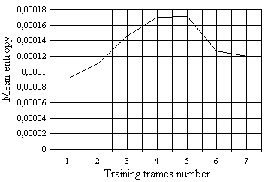
\includegraphics[width=\textwidth]{Figure2}
    \caption{Mean Entropy.}
    \label{fig:fig3a}
  \end{subfigure}%
  ~ %add desired spacing between images, e. g. ~, \quad, \qquad etc.
  % (or a blank line to force the subfigure onto a new line)
  \begin{subfigure}[b]{0.3\textwidth}
    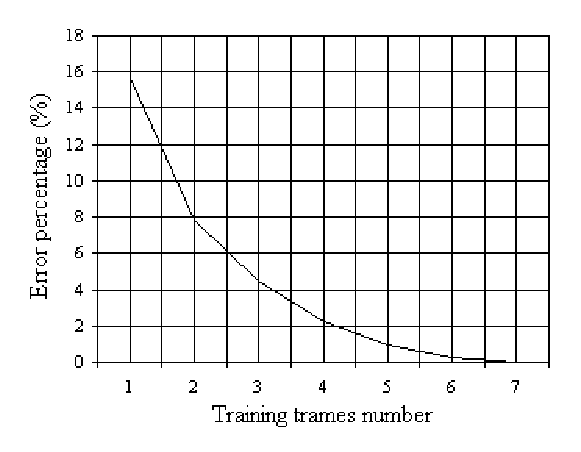
\includegraphics[width=\textwidth]{Figure3}
    \caption{Error Percentage.}
    \label{fig:fig3b}
  \end{subfigure}
  \caption{Optimal trames number in the training data set.}
  \label{fig:fig3}
\end{figure}

La figura~\ref{fig:LIdiapRoom} muestra otro ejemplo con referencias a las subfigures en el caption principal.

\begin{figure}
  \centering
  \begin{subfigure}[b]{0.30\textwidth}
    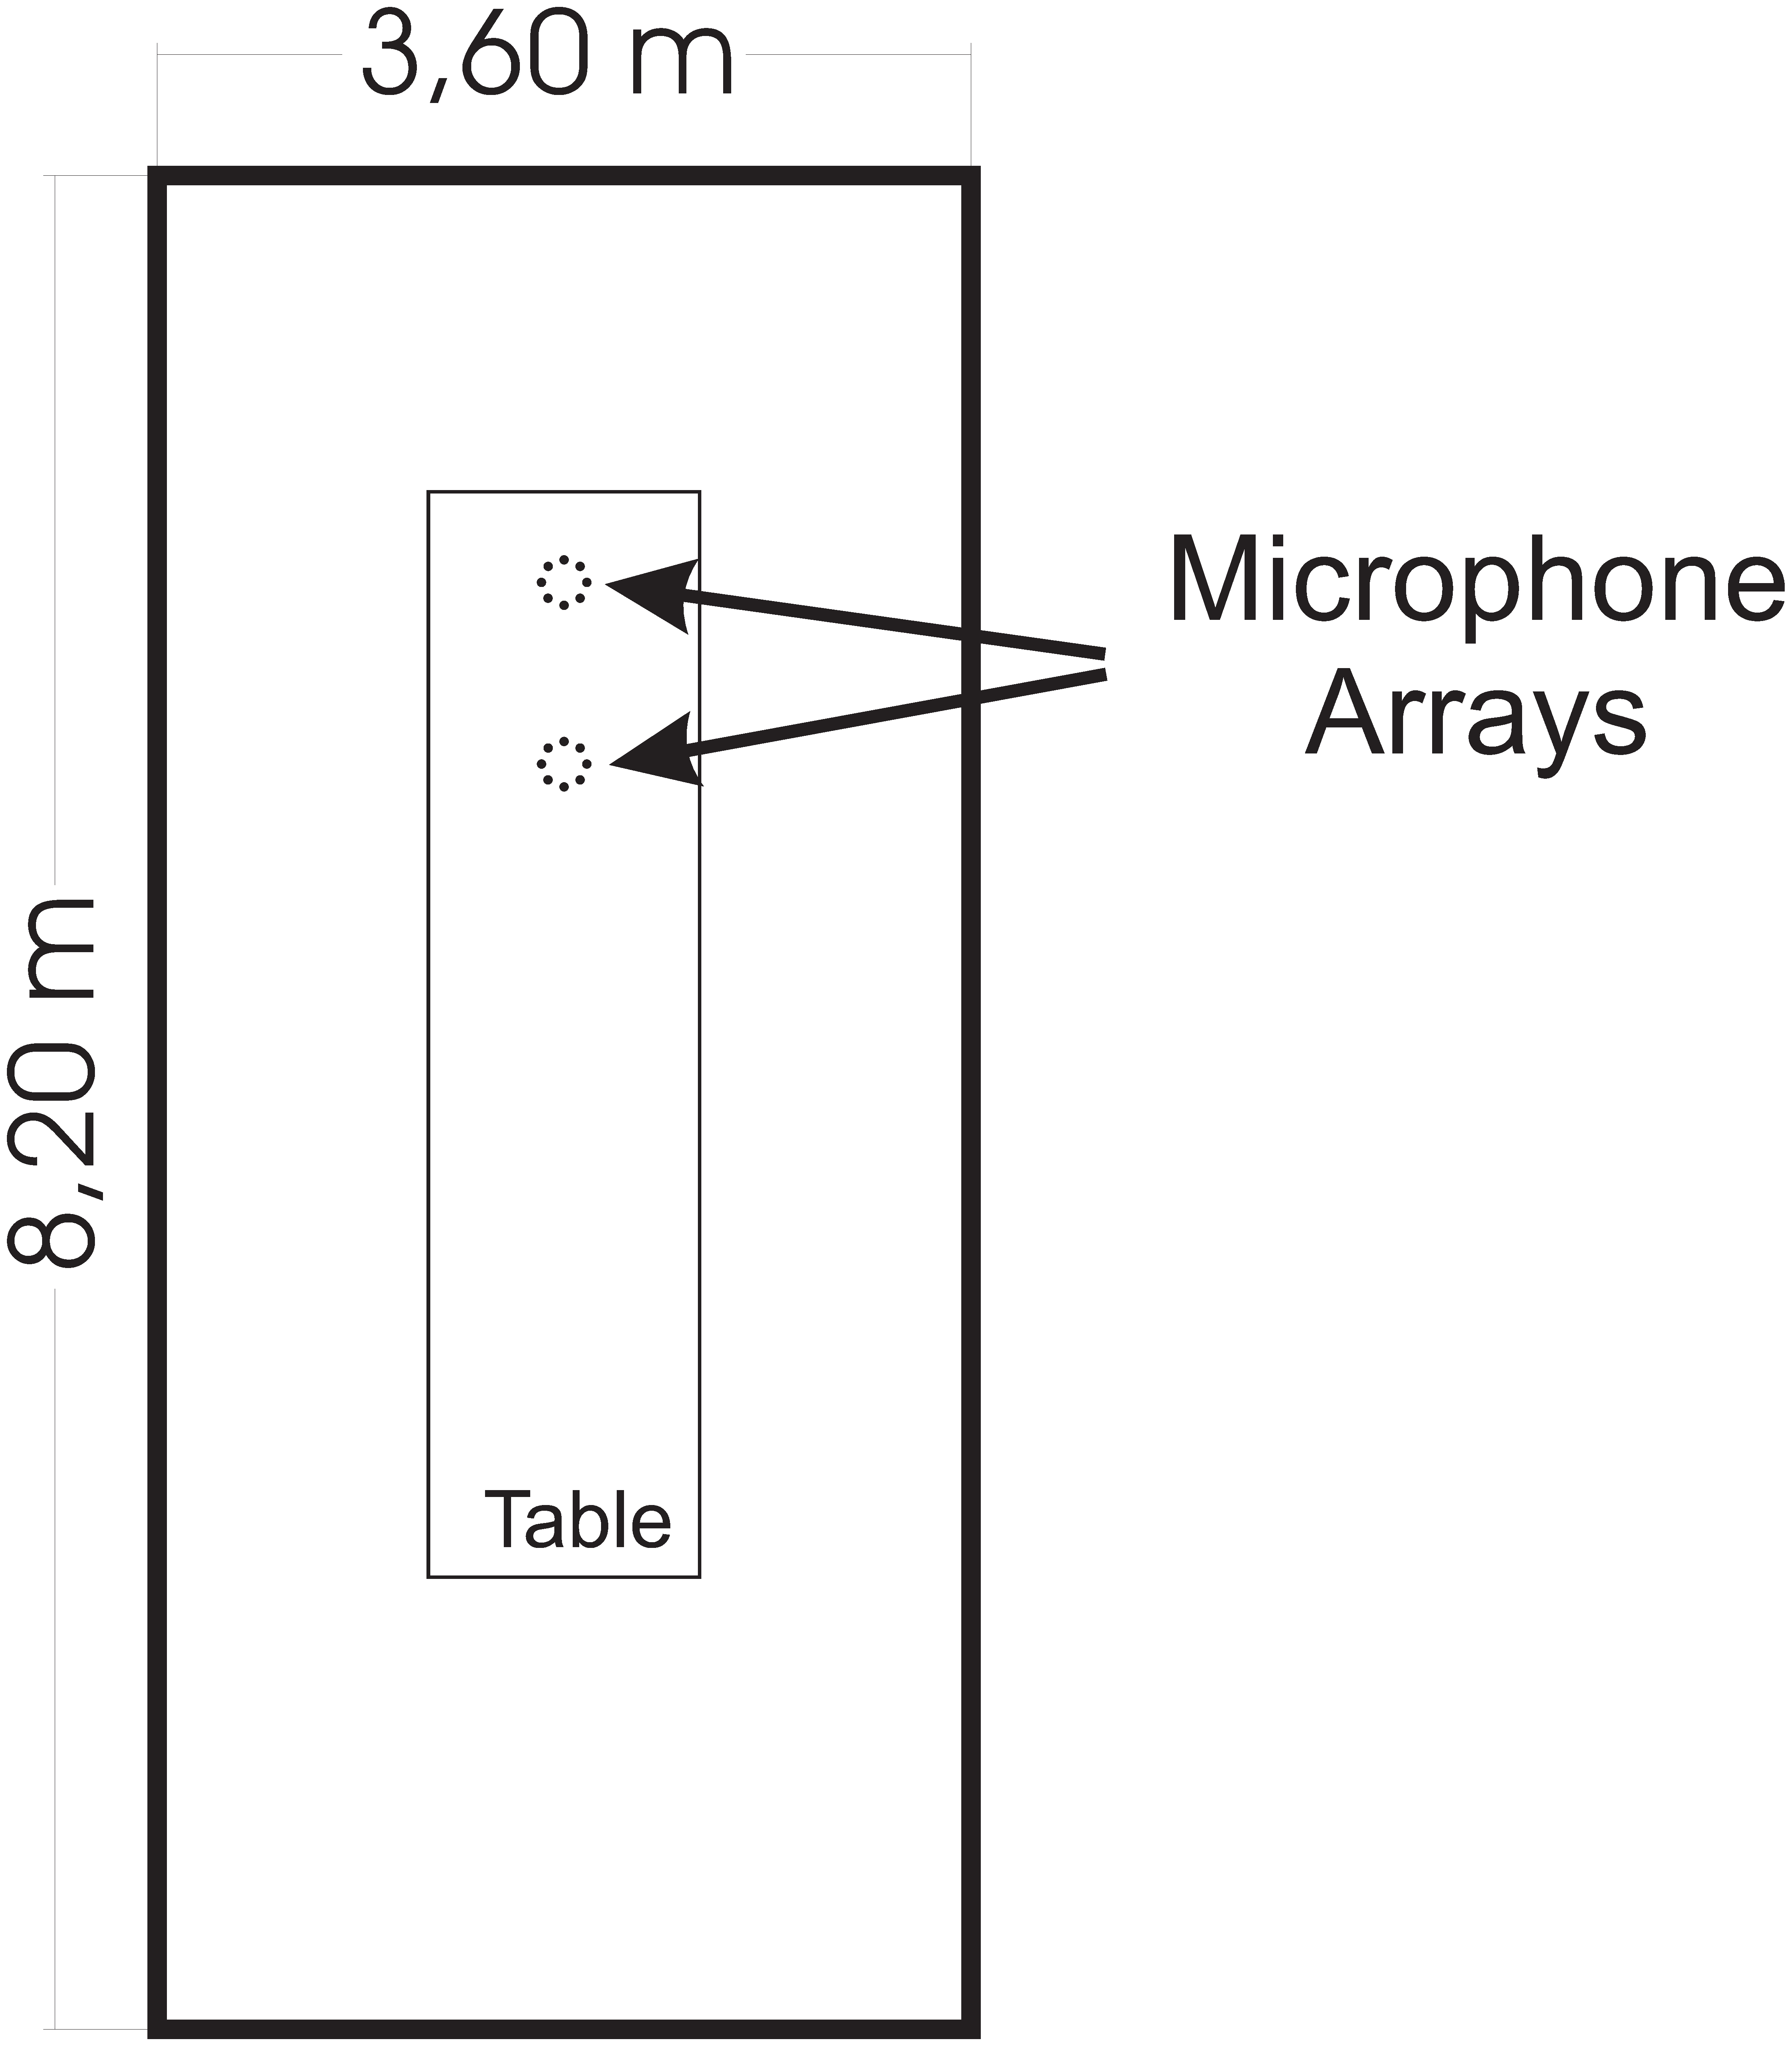
\includegraphics[width=\textwidth]{roomlayout2}
    \caption{}
    \label{fig:RoomLayout}
  \end{subfigure}%
  \qquad \qquad %add desired spacing between images, e. g. ~, \quad, \qquad, \hfill etc.
  % (or a blank line to force the subfigure onto a new line)
  \begin{subfigure}[b]{0.425\textwidth}
    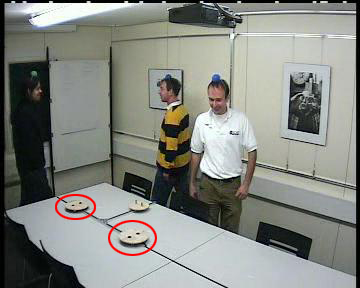
\includegraphics[width=\textwidth]{idiap-seq45-cam2.jpg}
    \caption{}
    \label{fig:RoomPicture}
  \end{subfigure}
  \caption{Idiap Smart Meeting Room for AV16.3 recordings. (\protect\subref{fig:RoomLayout}) Room layout showing the centered table, and the microphones arranged in two circular arrays. (\protect\subref{fig:RoomPicture}) Sample of recorded video frame showing the arrays area. \vspace{-0.3cm}}
  \label{fig:LIdiapRoom}
\end{figure}

Os incluimos a continuación un párrafo de un artículo en el que hacemos referencia a varias figuras y subfiguras:

\emph{The IDIAP Meeting Room (shown in figure~\ref{fig:LIdiapRoom}) is a $8.2m \times 3.6m \times 2.4m$ rectangular space containing a centrally located $4.8m \times 1.2m$ rectangular table, on top of which two circular microphone arrays of $10 cm$ radius are located, each of them composed by 8 microphones. The centers of the two arrays are separated by $80 cm$ and the origin of coordinates is located in the middle point between the two arrays. The arrays can be also seen in figures~\ref{fig:simureal_positions}.\subref{fig:Simulated_positions}, ~\ref{fig:simureal_positions}.\subref{fig:real_positions_short}, and ~\ref{fig:simureal_positions}.\subref{fig:real_positions_long}, in which only the relevant section of the room is displayed, each one showing different scenarios that were used in the experiments. A detailed description of the meeting room can be found in~\cite{moore2002}.}

\begin{figure}
  \centering
  \begin{subfigure}[t]{0.3\textwidth}
    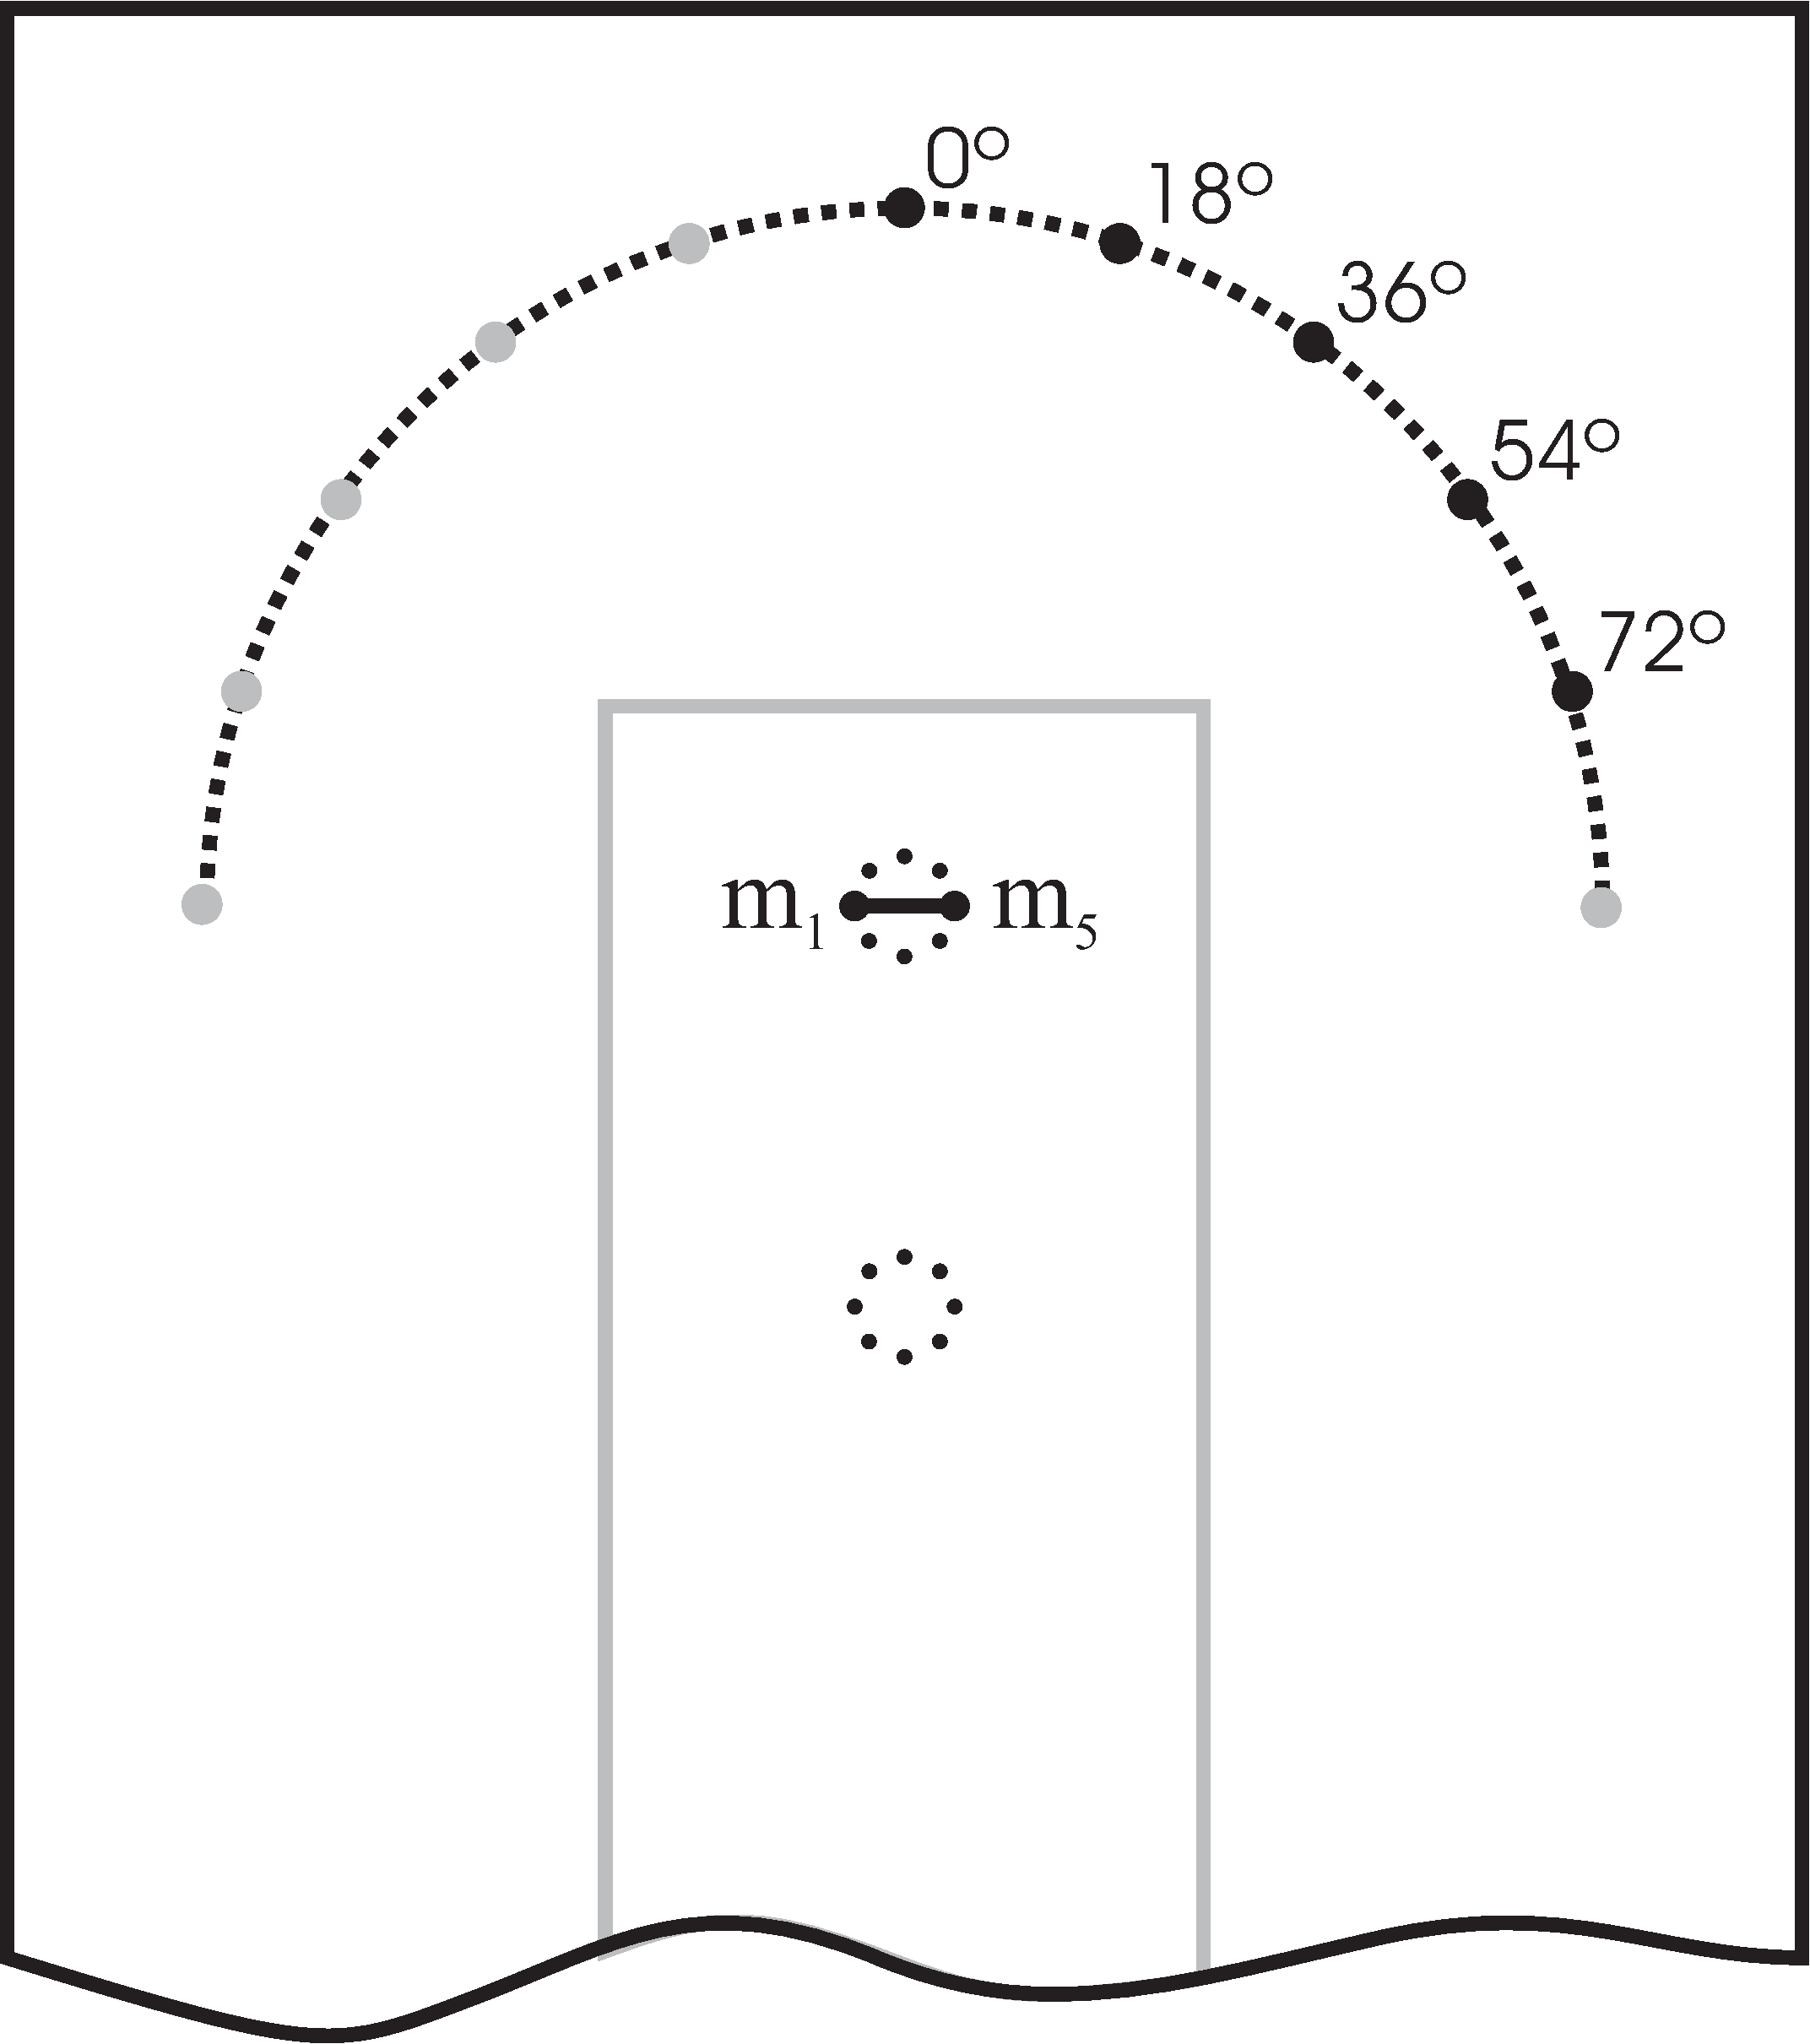
\includegraphics[width=\textwidth]{angular2-short-improved}
    \caption{For validation\\with simulated data.}
    \label{fig:Simulated_positions}
  \end{subfigure}
~%add desired spacing between images, e. g. ~, \quad, \qquad,
  % \hfill etc.
  % (or a blank line to force the subfigure onto a new line)
  \begin{subfigure}[t]{0.3\textwidth}
    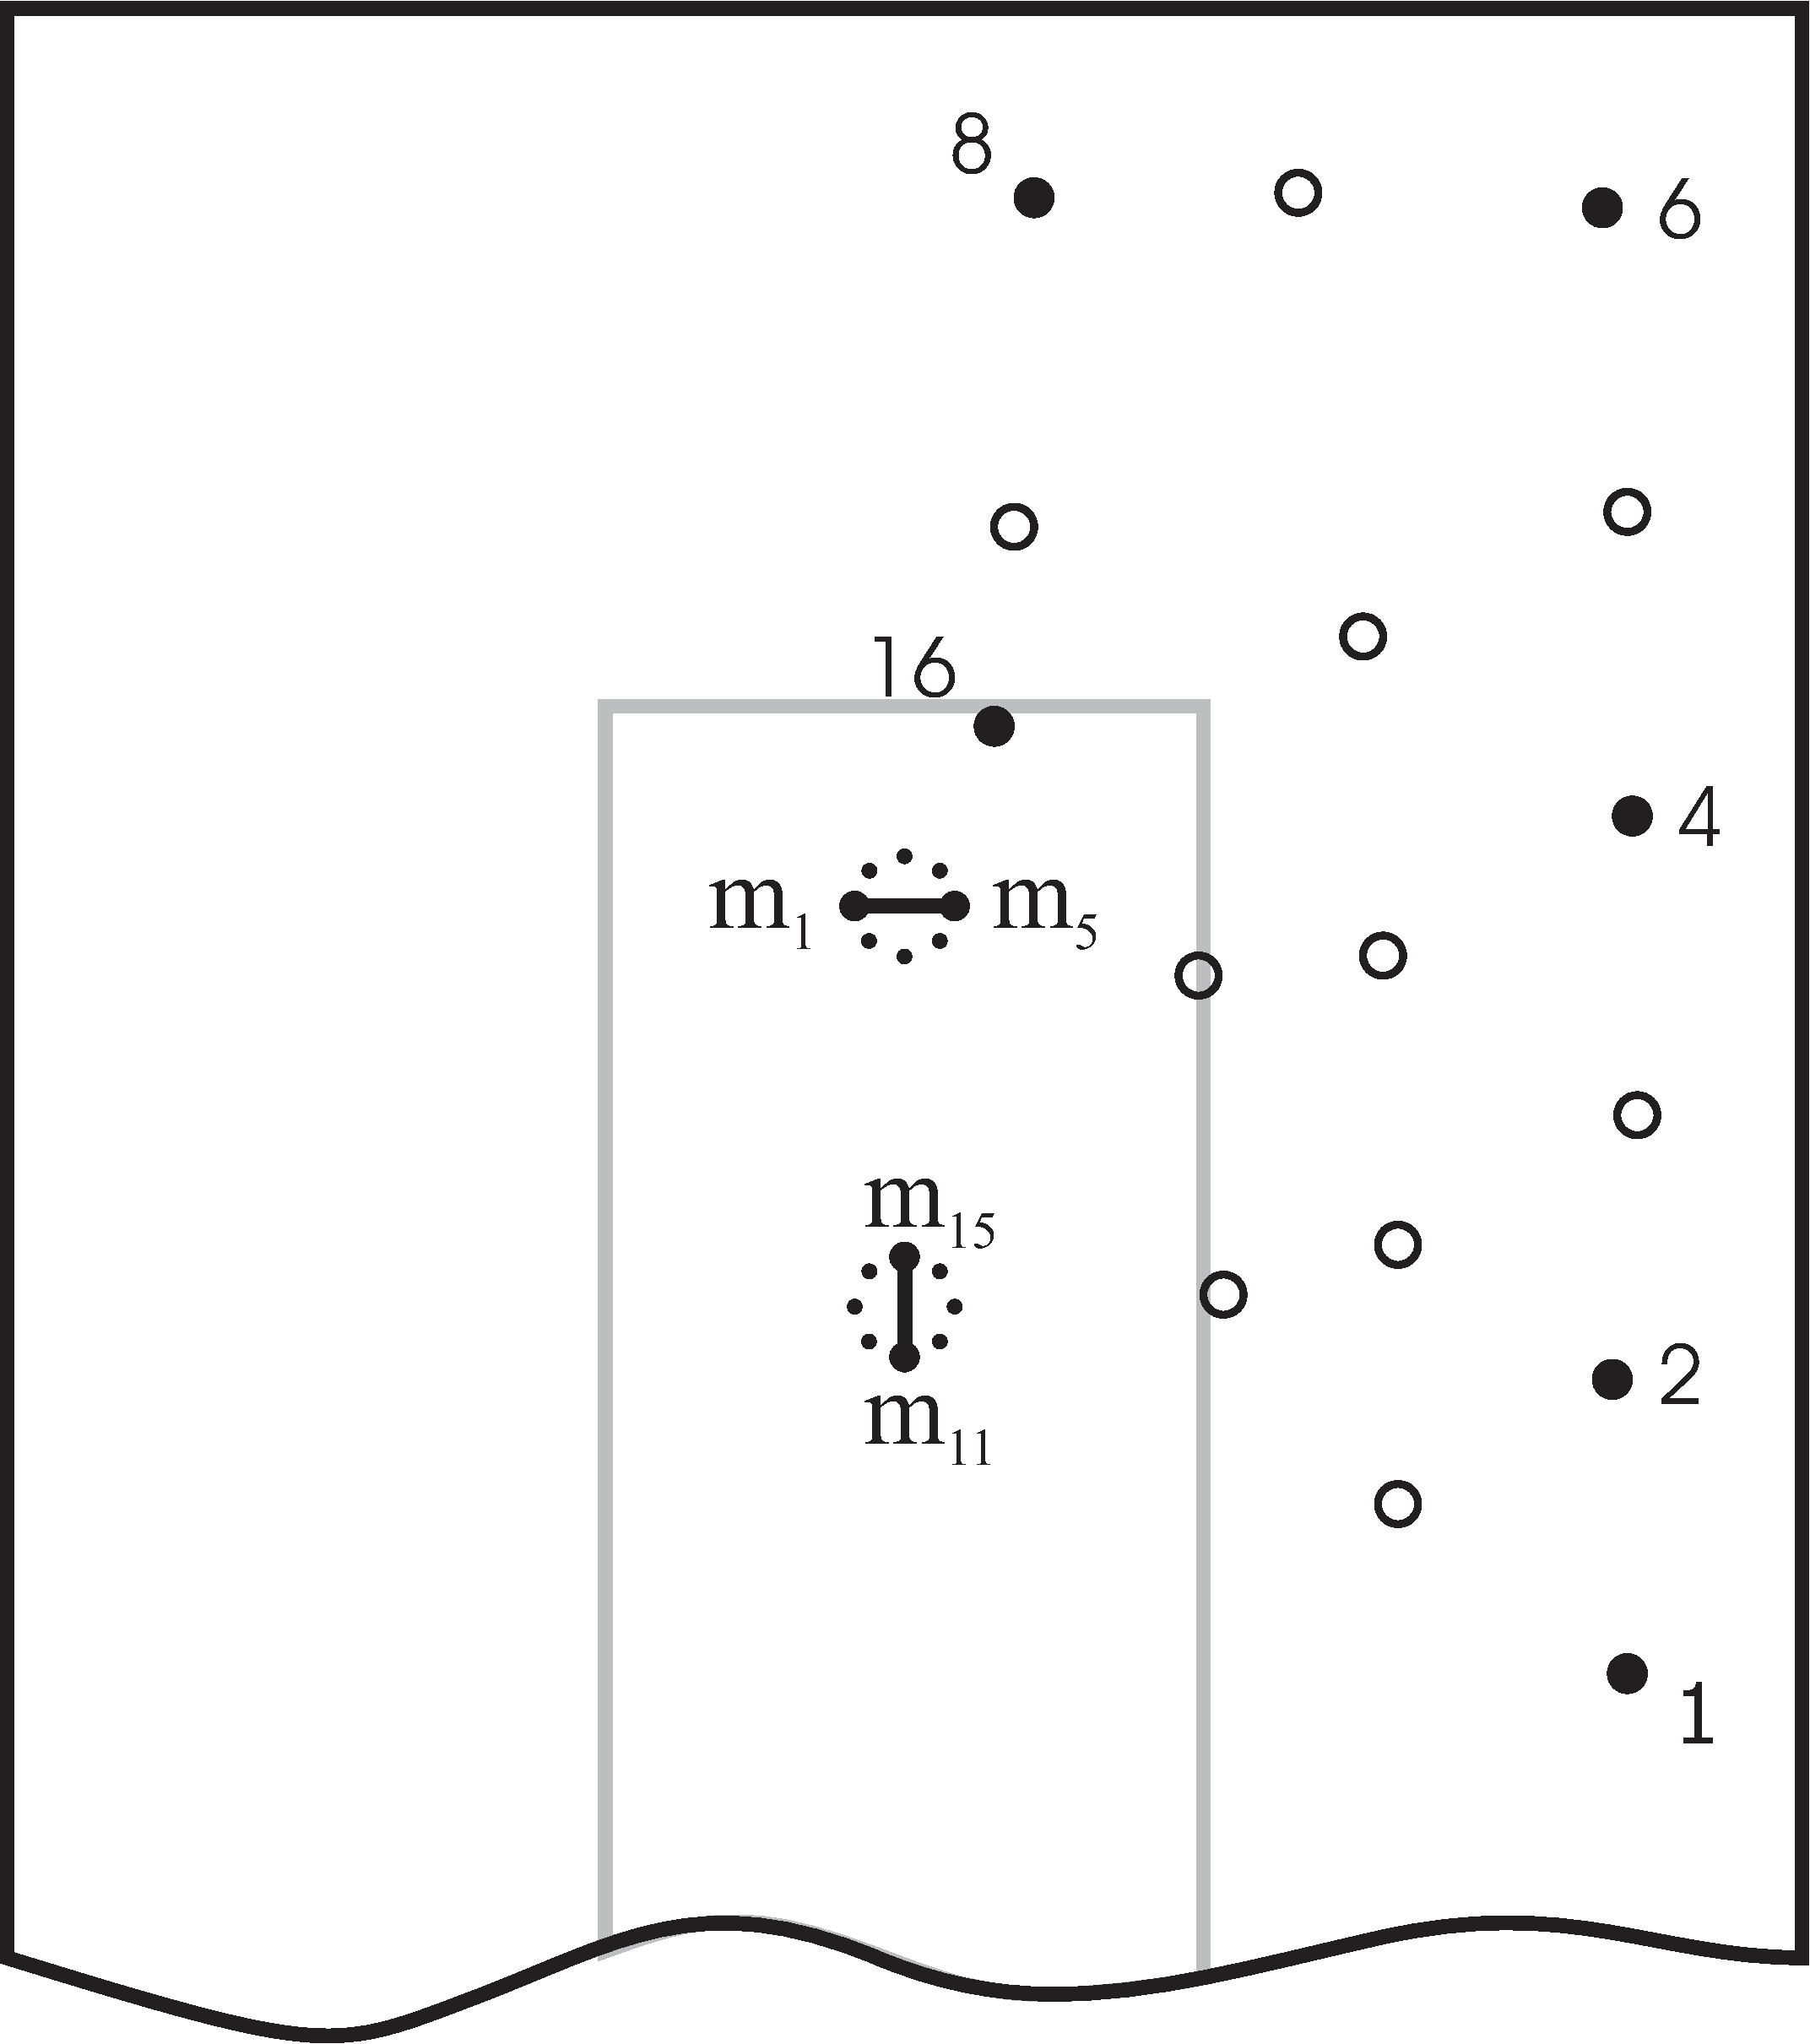
\includegraphics[width=\textwidth]{positions1-short-improved}
    \caption{For validation\\with real data and microphone pairs with $20~cm$ spacing.}
    \label{fig:real_positions_short}
  \end{subfigure}
  ~
  \begin{subfigure}[t]{0.3\textwidth}
    
\includegraphics[width=\textwidth]{positions2-short-improved}
    \caption{For validation\\with real data and microphone pairs with
      $82.46~cm$ spacing.}
    \label{fig:real_positions_long}
  \end{subfigure}
  \caption{Geometrical details for the experiments carried out. Only the
    relevant section of the room is shown, and microphone pairs are
    connected by solid lines.}
  \label{fig:simureal_positions}
\end{figure}

En la figura~\ref{fig:Sim_angles} mostramos un ejemplo de varias
figuras organizadas de forma un poco más complejo.

\begin{figure}
  \centering
  \begin{subfigure}[b]{0.3\textwidth}
    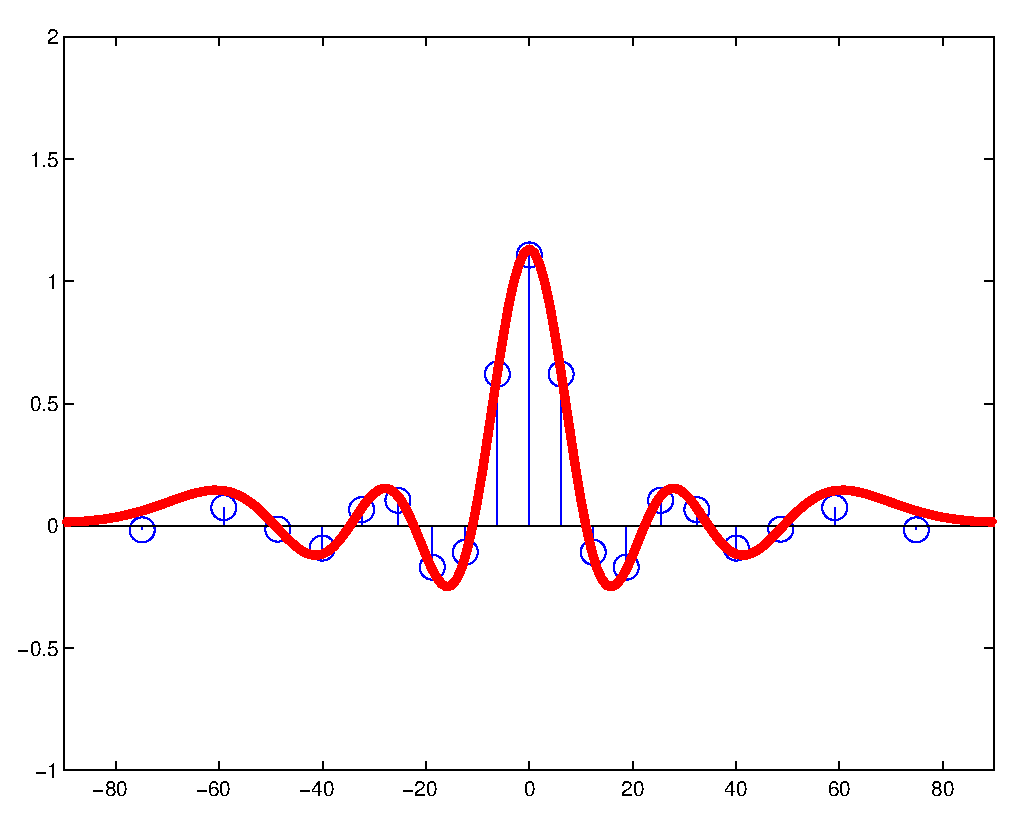
\includegraphics[width=\textwidth]{Sim_seg025_ang090}
    \caption{$0^{\circ}$}
    \label{fig:Sim_ang090}
  \end{subfigure}
  % add desired spacing between images, e. g. ~, \quad, \qquad etc.
  % (or a blank line to force the subfigure onto a new line)

  \begin{subfigure}[b]{0.3\textwidth}
    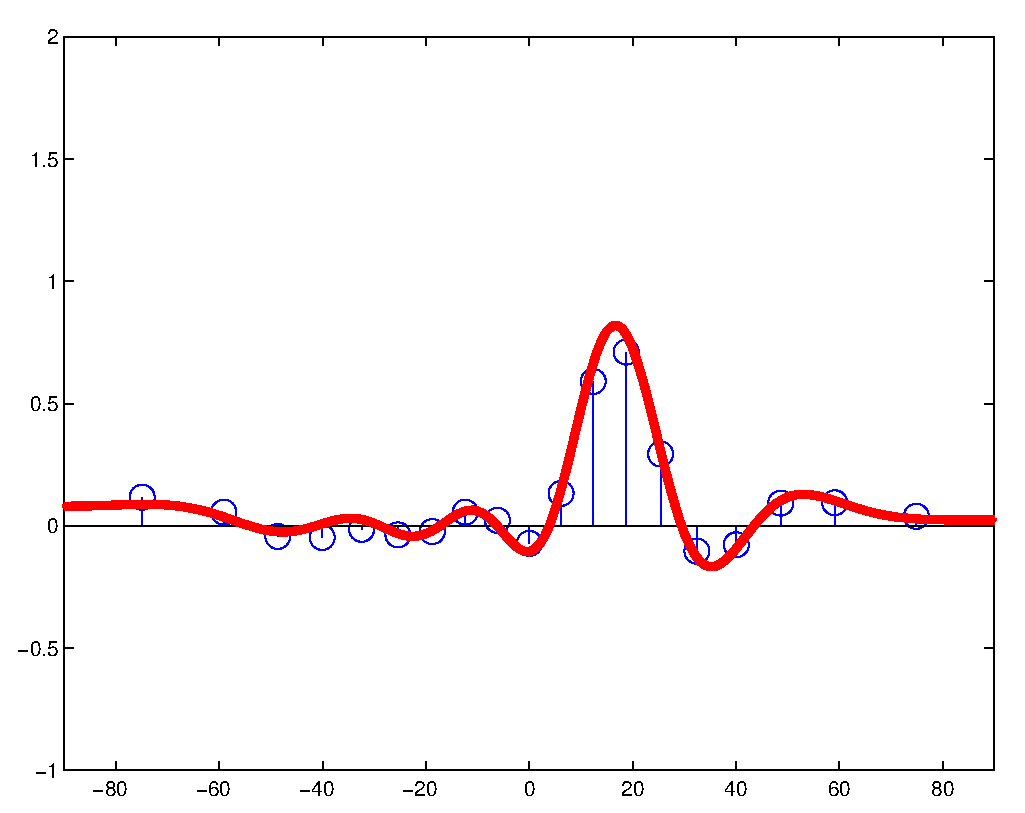
\includegraphics[width=\textwidth]{Sim_seg025_ang108}
    \caption{$18^{\circ}$}
    \label{fig:Sim_ang108}
  \end{subfigure}
  % add desired spacing between images, e. g. ~, \quad, \qquad etc.
  % (or a blank line to force the subfigure onto a new line)
  \begin{subfigure}[b]{0.3\textwidth}
    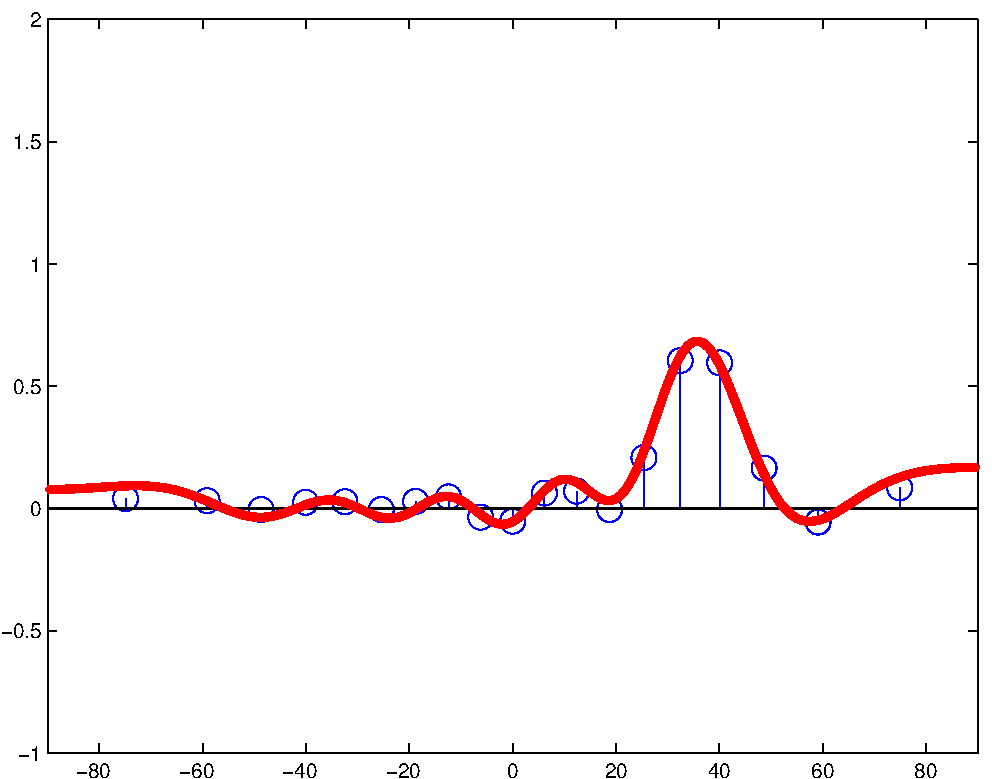
\includegraphics[width=\textwidth]{Sim_seg025_ang126}
    \caption{$36^{\circ}$}
    \label{fig:Sim_ang126}
  \end{subfigure}
  % add desired spacing between images, e. g. ~, \quad, \qquad etc.
  % (or a blank line to force the subfigure onto a new line)
  \begin{subfigure}[b]{0.3\textwidth}
    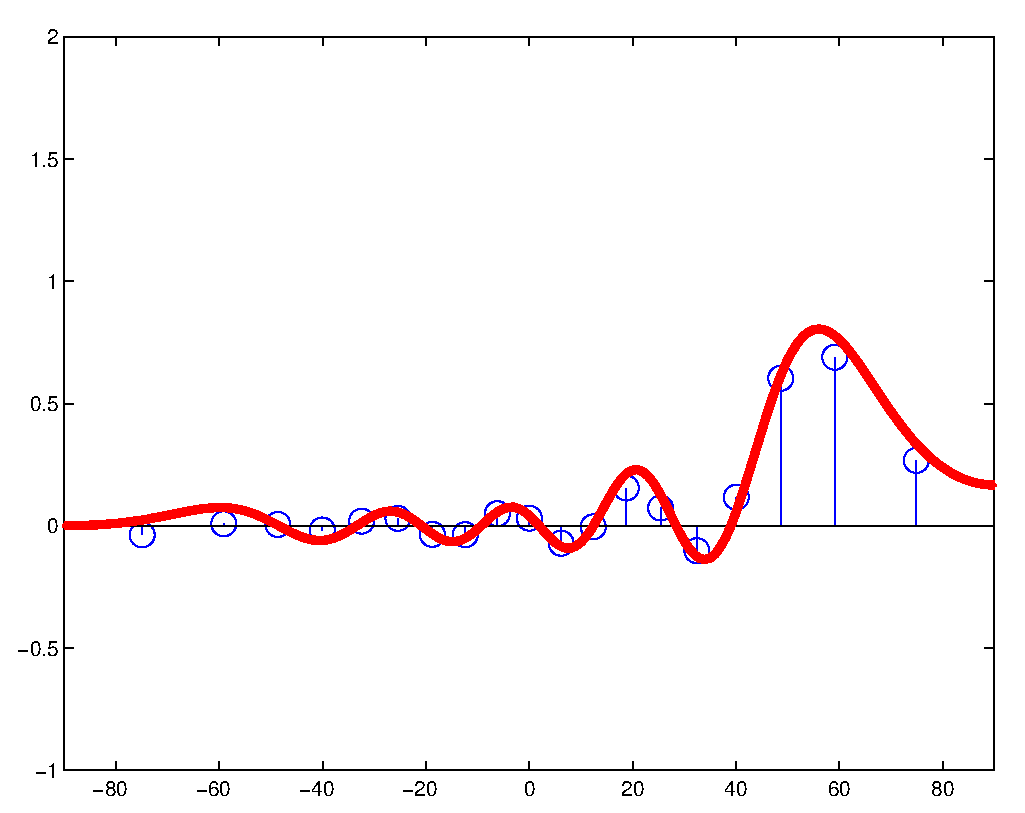
\includegraphics[width=\textwidth]{Sim_seg025_ang144}
    \caption{$54^{\circ}$}
    \label{fig:Sim_ang144}
  \end{subfigure}
  % add desired spacing between images, e. g. ~, \quad, \qquad etc.
  % (or a blank line to force the subfigure onto a new line)

  \begin{subfigure}[b]{0.3\textwidth}
    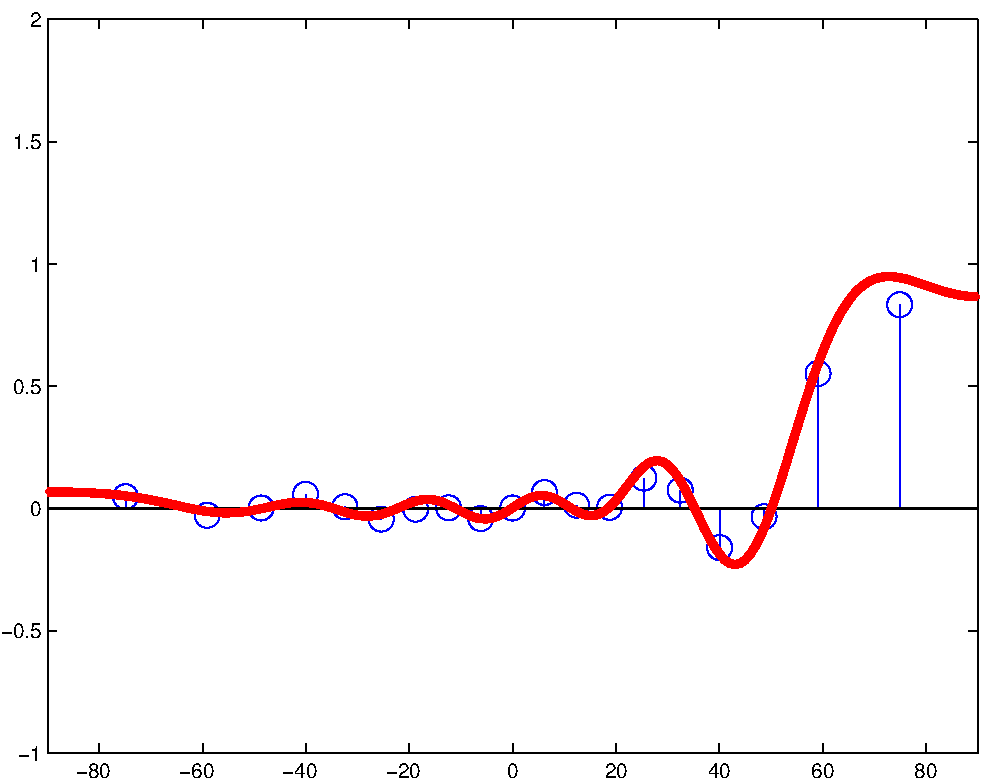
\includegraphics[width=\textwidth]{Sim_seg025_ang162}
    \caption{$72^{\circ}$}
    \label{fig:Sim_ang162}
  \end{subfigure}

  \caption{Comparison between the steered power response generated by the model (solid line) and that calculated using simulated waveforms in the AV16.3 environment (stems). Results for the speaker in given angles and the array steered from -90º to +90º are shown.}
  \label{fig:Sim_angles}
\end{figure}

También es posible incluir el código de una figura en un fichero \texttt{.tex} independiente (para hacer más legible el código del documento principal). Un ejemplo lo tenéis a continuación, incluyendo el texto en inglés del documento original:

\emph{Figure~\ref{fig:SRPvsPatternSelected} includes the results of the comparison, for several speaker positions (1, 2, 4, 6, 8 and 16, emphasized in figure~\ref{fig:simureal_positions}.\subref{fig:real_positions_short}), and selected to provide different acoustic situations, both in terms of distance and angular position with respect to the arrays. All the graphics show the acoustic power map (predicted or calculated) for a regular two-dimensional grid of $10~cm$. The plot is provided from a top view of the room, spanning the full plan at a height of $61~cm$ above the microphone arrays (this height was the ground truth one for sequence 01). For each speaker position shown, three graphics are plotted:}

\begin{itemize}
  \item \emph{The graphics on the left show the SRP-PHAT acoustic power maps generated by the proposed model (for example, the left graphic in figure~\ref{fig:SRPvsPatternSelected}.\subref{fig:SRPvsModel_Fo1500_position1} for position 1).}
  \item \emph{The graphics in the middle show the real SRP-PHAT acoustic power maps calculated using the real acoustic waveforms (for example, the middle graphic in figure~\ref{fig:SRPvsPatternSelected}.\subref{fig:SRPvsModel_Fo1500_position1} for position 1), for a single selected frame.}
  \item \emph{The graphics on the right show the average real SRP-PHAT acoustic power maps, averaging for all the frames in which the user was in the given position (for example, the right graphic in figure~\ref{fig:SRPvsPatternSelected}.\subref{fig:SRPvsModel_Fo1500_position1} for position 1).}
\end{itemize}

\emph{The green point represents the real (ground truth) speaker position, and the black dots represent the positions of the four microphones used. The hyperbolic shapes found in the figure are consistent with the fact that the place of points with equal acoustic power value, for a given microphone pair, is a hyperbola (in our two-dimensional case, being a hyperboloid of revolution in the three-dimensional case).}

\emph{From figure~\ref{fig:SRPvsPatternSelected}, it can clearly be seen that, again, the predictions closely match the results with real data for the different acoustic conditions, even when the simulations are using fixed and frequency independent average reflection coefficients, and that the acoustic model is based on the simplistic image method model.}

\begin{figure}
  \centering
  \begin{subfigure}[t]{0.47\textwidth}
    \begin{minipage}[t]{\textwidth}
      \begin{subfigure}[t]{0.3\textwidth}
        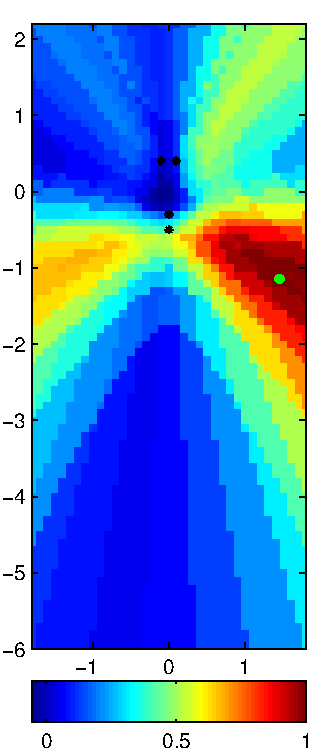
\includegraphics[width=\textwidth]{Pattern_Fo1500_pos01}
        %\caption{SRP Model for pos. 1}
        \label{fig:Pattern_Fo1500_pos01}
      \end{subfigure}
      % ~ %add desired spacing between images, e. g. ~, \quad, \qquad,
      % \hfill etc.
      % (or a blank line to force the subfigure onto a new line)
      \begin{subfigure}[t]{0.3\textwidth}
        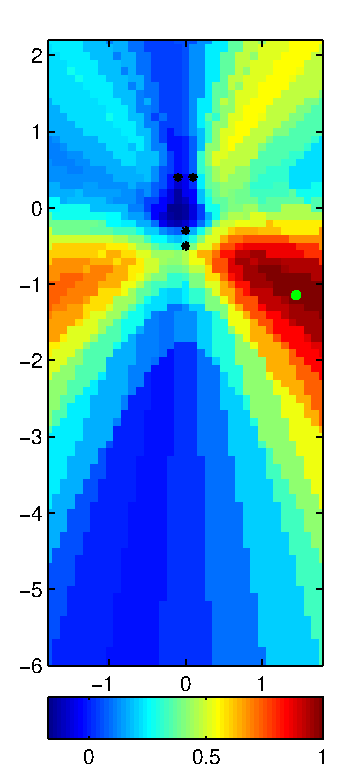
\includegraphics[width=\textwidth]{SRP_Fo1500_frame003_pos01}
        % \caption{Real SRP for pos.  1}
        \label{fig:SRP_Fo1500_pos01}
      \end{subfigure}
      % ~ %add desired spacing between images, e. g. ~, \quad, \qquad,
      % \hfill etc.
      % (or a blank line to force the subfigure onto a new line)
      \begin{subfigure}[t]{0.3\textwidth}
        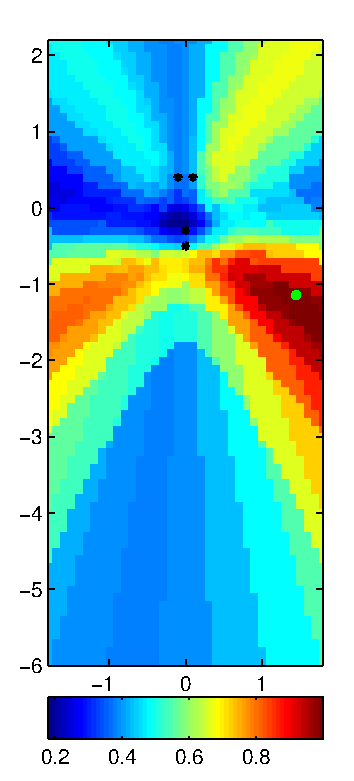
\includegraphics[width=\textwidth]{SRP_Fo1500_mean_pos01}
        % \caption{Avg. SRP for pos. 1}
        \label{fig:SRP_Fo1500_mean_pos01}
      \end{subfigure}
      \vspace{\verticalSpacingSRPMaps}
      \caption{\centering For position 1}
      \label{fig:SRPvsModel_Fo1500_position1}
      \vspace{0.25cm}
    \end{minipage}
  \end{subfigure}
  ~% \quad % between 1 and 2 %add desired spacing between images, e. g. ~, \quad, \qquad,
  % \hfill etc.
  % (or a blank line to force the subfigure onto a new line)
  \begin{subfigure}[t]{0.47\textwidth}
    \begin{minipage}[t]{\textwidth}
      \begin{subfigure}[t]{0.3\textwidth}
        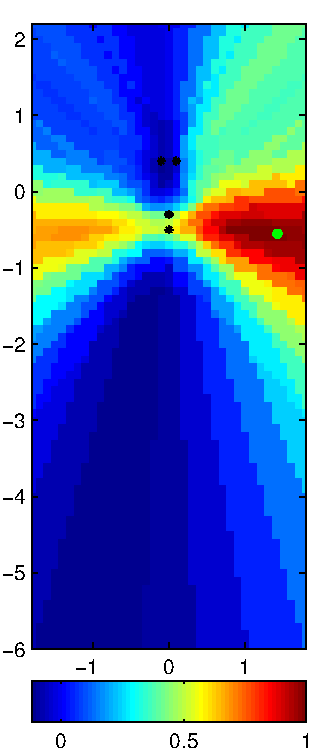
\includegraphics[width=\textwidth]{Pattern_Fo1500_pos02}
        % \caption{SRP Model for pos. 2}
        \label{fig:Pattern_Fo1500_pos02}
      \end{subfigure}
      % ~ %add desired spacing between images, e. g. ~, \quad, \qquad,
      % \hfill etc.
      % (or a blank line to force the subfigure onto a new line)
      \begin{subfigure}[t]{0.3\textwidth}
        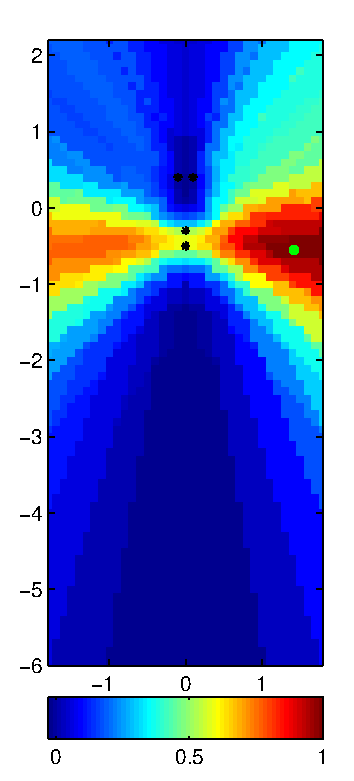
\includegraphics[width=\textwidth]{SRP_Fo1500_frame161_pos02}
        % \caption{Real SRP for pos.  2\\}
        \label{fig:SRP_pos02}
      \end{subfigure}
      % ~ %add desired spacing between images, e. g. ~, \quad, \qquad,
      % \hfill etc.
      % (or a blank line to force the subfigure onto a new line)
      \begin{subfigure}[t]{0.3\textwidth}
        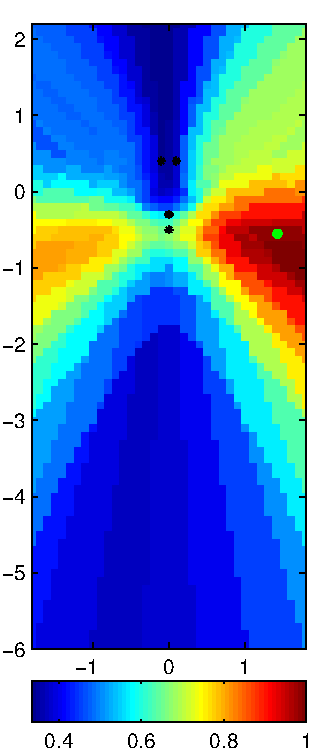
\includegraphics[width=\textwidth]{SRP_Fo1500_mean_pos02}
        % \caption{Avg. SRP for pos. 2}
        \label{fig:SRP_Fo1500_mean_pos02}
      \end{subfigure}
      \vspace{\verticalSpacingSRPMaps}
      \caption{\centering For position 2}
      \vspace{0.25cm}
    \end{minipage}
  \end{subfigure}

  \begin{subfigure}[t]{0.47\textwidth}
    \begin{minipage}[t]{\textwidth}
      \begin{subfigure}[t]{0.3\textwidth}
        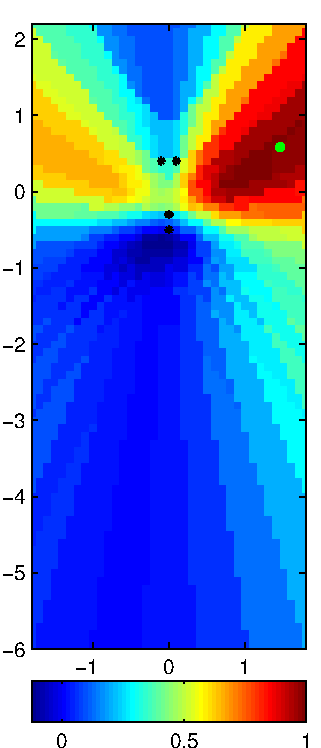
\includegraphics[width=\textwidth]{Pattern_Fo1500_pos04}
        % \caption{SRP Model for pos. 4}
        \label{fig:Pattern_Fo1500_pos04}
      \end{subfigure}
      % ~ %add desired spacing between images, e. g. ~, \quad, \qquad,
      % \hfill etc.
      % (or a blank line to force the subfigure onto a new line)
      \begin{subfigure}[t]{0.3\textwidth}
        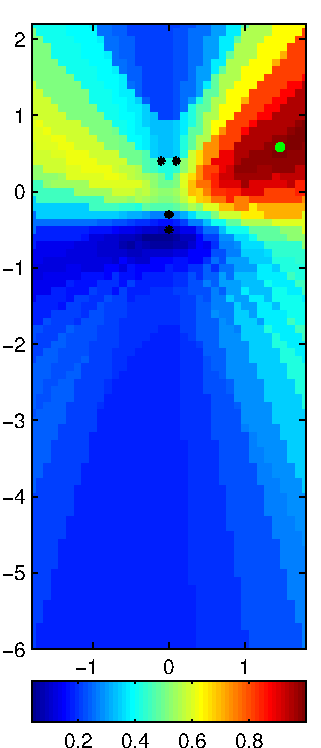
\includegraphics[width=\textwidth]{SRP_Fo1500_frame464_pos04}
        % \caption{Real SRP for pos.  4\\}
        \label{fig:SRP_pos04}
      \end{subfigure}
      % ~ %add desired spacing between images, e. g. ~, \quad, \qquad,
      % \hfill etc.
      % (or a blank line to force the subfigure onto a new line)
      \begin{subfigure}[t]{0.3\textwidth}
        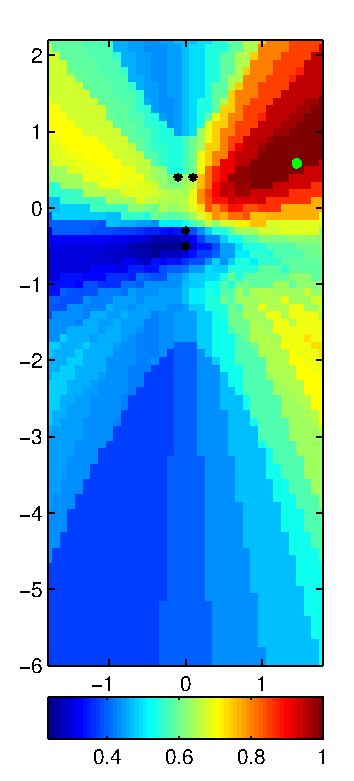
\includegraphics[width=\textwidth]{SRP_Fo1500_mean_pos04}
        % \caption{Avg. SRP for pos. 4}
        \label{fig:SRP_Fo1500_mean_pos04}
      \end{subfigure}
      \vspace{\verticalSpacingSRPMaps}
      \caption{\centering For position 4}
      \vspace{0.25cm}
    \end{minipage}
  \end{subfigure}
  ~%  \qquad % between 4 and 6 %add desired spacing between images, e. g. ~, \quad, \qquad,
  % \hfill etc.
  % (or a blank line to force the subfigure onto a new line)
  \begin{subfigure}[t]{0.47\textwidth}
    \begin{minipage}[t]{\textwidth}
      \begin{subfigure}[t]{0.3\textwidth}
        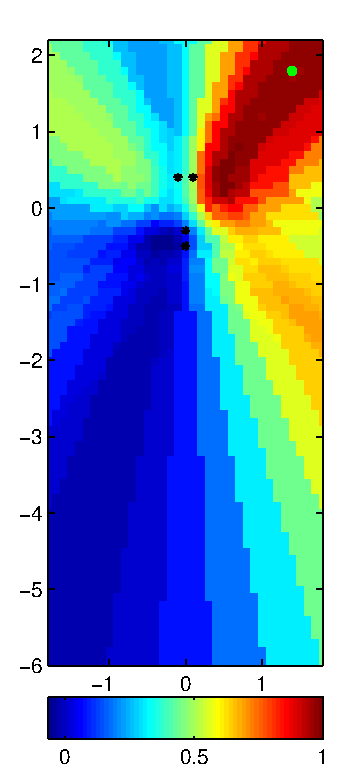
\includegraphics[width=\textwidth]{Pattern_Fo1500_pos06}
        % \caption{SRP Model for pos. 6}
        \label{fig:Pattern_Fo1500_pos06}
      \end{subfigure}
      % ~ %add desired spacing between images, e. g. ~, \quad, \qquad,
      % \hfill etc.
      % (or a blank line to force the subfigure onto a new line)
      \begin{subfigure}[t]{0.3\textwidth}
        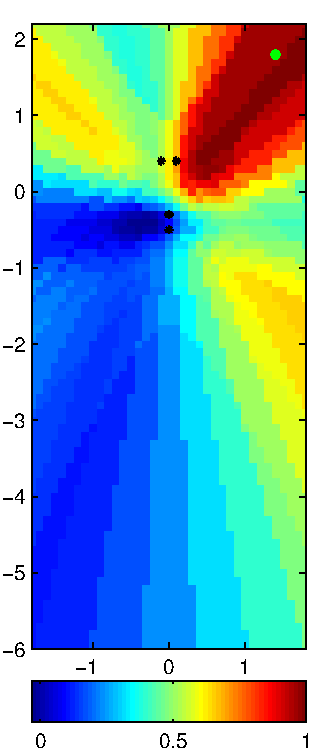
\includegraphics[width=\textwidth]{SRP_Fo1500_frame809_pos06}
        % \caption{Real SRP for pos.  6\\}
        \label{fig:SRP_pos06}
      \end{subfigure}
      % ~ %add desired spacing between images, e. g. ~, \quad, \qquad,
      % \hfill etc.
      % (or a blank line to force the subfigure onto a new line)
      \begin{subfigure}[t]{0.3\textwidth}
        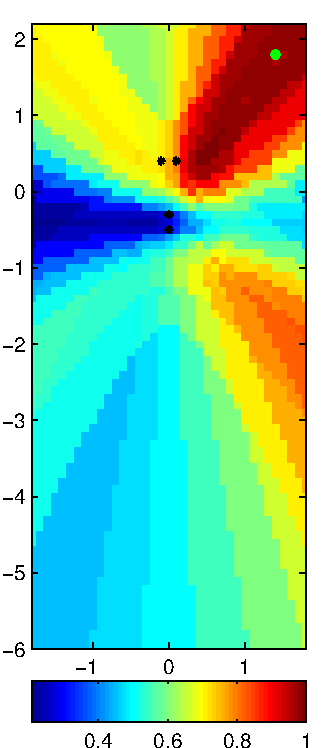
\includegraphics[width=\textwidth]{SRP_Fo1500_mean_pos06}
        % \caption{Avg. SRP for pos. 6}
        \label{fig:SRP_Fo1500_mean_pos06}
      \end{subfigure}
      \vspace{\verticalSpacingSRPMaps}
      \caption{\centering For position 6}
      \vspace{0.25cm}
    \end{minipage}
  \end{subfigure}

  \begin{subfigure}[t]{0.47\textwidth}
    \begin{minipage}[t]{\textwidth}
      \begin{subfigure}[t]{0.3\textwidth}
        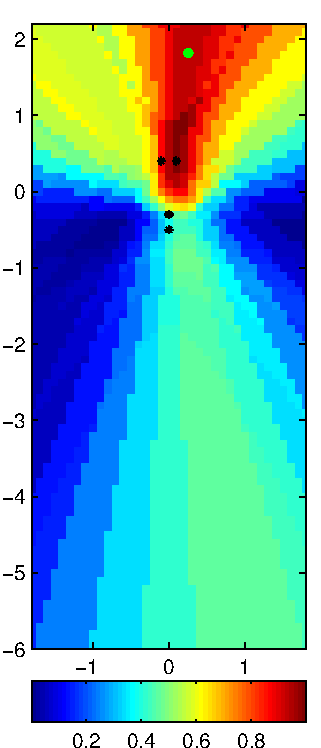
\includegraphics[width=\textwidth]{Pattern_Fo1500_pos08}
        % \caption{SRP Model for pos. 8}
        \label{fig:Pattern_Fo1500_pos08}
      \end{subfigure}
      % ~ %add desired spacing between images, e. g. ~, \quad, \qquad,
      % \hfill etc.
      % (or a blank line to force the subfigure onto a new line)
      \begin{subfigure}[t]{0.3\textwidth}
        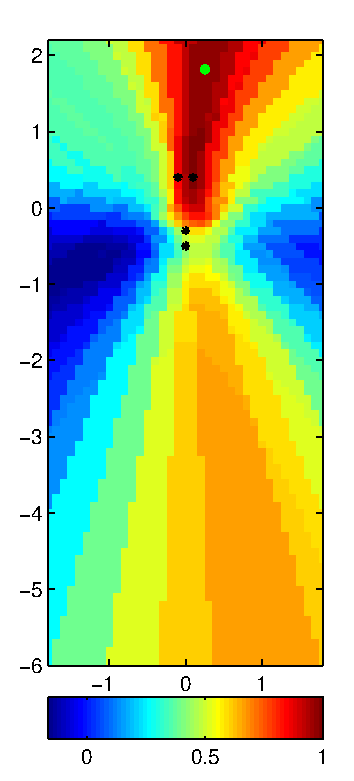
\includegraphics[width=\textwidth]{SRP_Fo1500_frame1127_pos08}
        % \caption{Real SRP for pos.  8\\}
        \label{fig:SRP_pos08}
      \end{subfigure}
      % ~ %add desired spacing between images, e. g. ~, \quad, \qquad,
      % \hfill etc.
      % (or a blank line to force the subfigure onto a new line)
      \begin{subfigure}[t]{0.3\textwidth}
        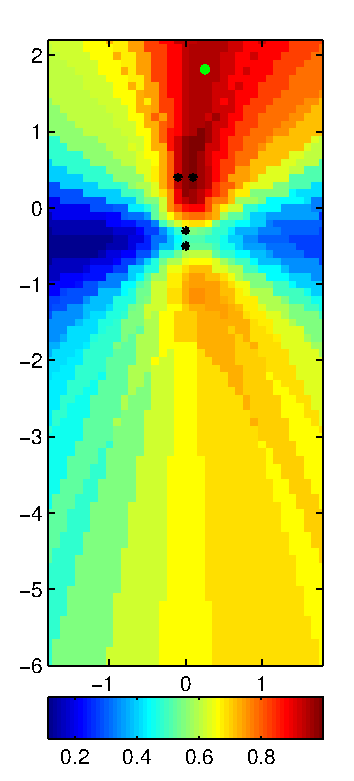
\includegraphics[width=\textwidth]{SRP_Fo1500_mean_pos08}
        % \caption{Avg. SRP for pos. 8}
        \label{fig:SRP_Fo1500_mean_pos08}
      \end{subfigure}
      \vspace{\verticalSpacingSRPMaps}
      \caption{\centering For position 8}
      \vspace{0.25cm}
    \end{minipage}
  \end{subfigure}
  ~%  \qquad % between 8 and 16 %add desired spacing between images, e. g. ~, \quad, \qquad,
  % \hfill etc.
  % (or a blank line to force the subfigure onto a new line)
  \begin{subfigure}[t]{0.47\textwidth}
    \begin{minipage}[t]{\textwidth}
      \begin{subfigure}[t]{0.3\textwidth}
        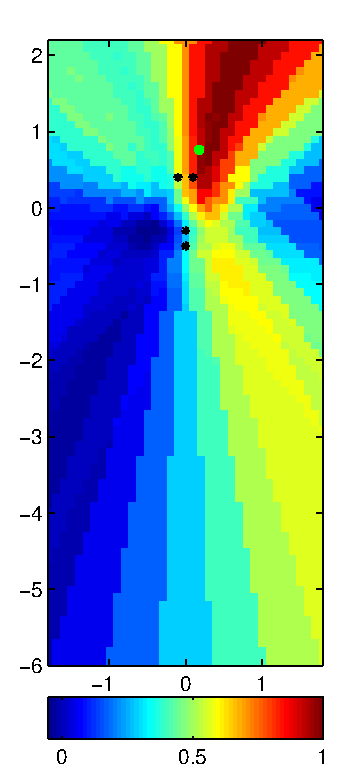
\includegraphics[width=\textwidth]{Pattern_Fo1500_pos16}
        % \caption{SRP Model for pos. 16}
        \label{fig:Pattern_Fo1500_pos16}
      \end{subfigure}
      % ~ %add desired spacing between images, e. g. ~, \quad, \qquad,
      % \hfill etc.
      % (or a blank line to force the subfigure onto a new line)
      \begin{subfigure}[t]{0.3\textwidth}
        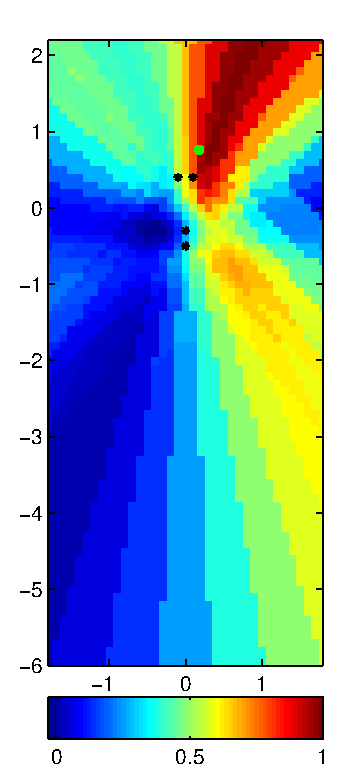
\includegraphics[width=\textwidth]{SRP_Fo1500_frame2518_pos16}
        % \caption{Real SRP for pos. 16\\}
        \label{fig:SRP_pos16}
      \end{subfigure}
      % ~ %add desired spacing between images, e. g. ~, \quad, \qquad,
      % \hfill etc.
      % (or a blank line to force the subfigure onto a new line)
      \begin{subfigure}[t]{0.3\textwidth}
        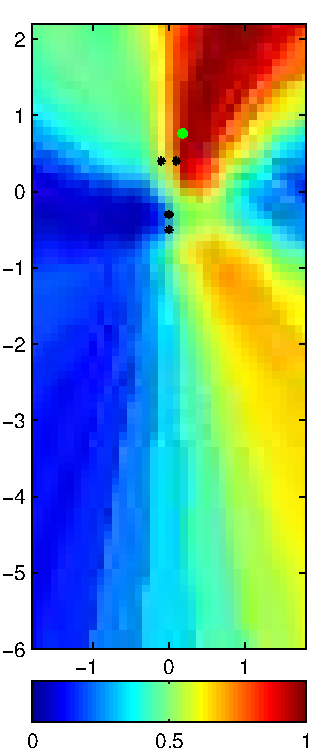
\includegraphics[width=\textwidth]{SRP_Fo1500_mean_pos16}
        % \caption{Avg. SRP for pos. 16}
        \label{fig:SRP_Fo1500_mean_pos16}
      \end{subfigure}
      \vspace{\verticalSpacingSRPMaps}
      \caption{\centering For position 16}
      \vspace{0.25cm}
    \end{minipage}
  \end{subfigure}
  \caption{Comparison between the SRP-PHAT map predicted by the model
    (left graphics),
    the real SRP-PHAT map (middle graphics), and the average (real)
    SRP-PHAT map (right graphics), for
    several speaker positions ($f_0=1.5~KHz$). See
    figure~~\ref{fig:simureal_positions}.\subref{fig:real_positions_short}
    for geometrical references.}
  \label{fig:SRPvsPatternSelected}
\end{figure}
 

\begin{wrapfigure}{r}{0.5\textwidth} 
\vspace{-20pt}
  \begin{center}
    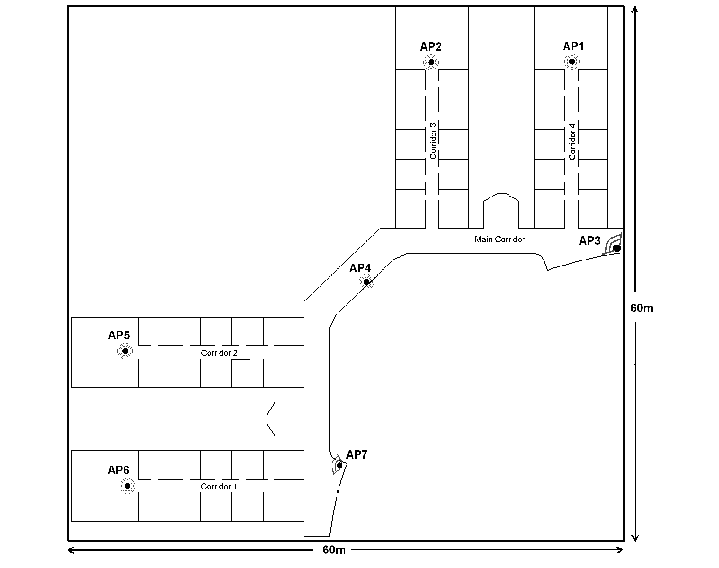
\includegraphics[width=0.4\textwidth]{Figure1}
    \caption{Ejemplo de figura con wrapfigure.}
    \label{fig:wrapfigure1}
  \end{center}
  \vspace{-20pt}
  \vspace{1pt}
\end{wrapfigure} 

Otra posibilidad es utilizar el entorno \texttt{wrapfig} para hacer que el texto bordee a las figuras, como en la figura~\ref{fig:wrapfigure1}. Añado ahora unas líneas de loren ipsum para que lo veáis bien. \lipsum[1-1]

% \lipsum[1-4]
% \begin{wrapfigure}{R}{5cm}
% \centering
% \rule{3cm}{7cm}
% \end{wrapfigure}
% \lipsum[1-6]

Incluso podemos poner una tabla ``apaisada'', como en la \ref{tab:tablas2006}, donde se muestra un resumen de los resultados obtenidos en una serie de experimentos de localización de locutores.

\clearpage
% \begin{table}[H]\centering
\begin{sidewaystable}[hbtp]
  \begin{center}

    \begin{tabular}{||l|c|c|c|c|c||}
      \hline \hline
      & UKA & ITC & AIT & UPC & IBM\\
      \hline
      \hline
      Pcor & $57.0\pm1.4\%$ & $84.0\pm3.3\%$ & $47.0\pm3.1\%$ & $20.0\pm2.5\%$ & $67.0\pm2.9\%$ \\
      \hline
      Bias fine (x:y:z) [mm] & $20:-42:-75$ & $45:27:-41$ & $-27:-77:-40$ & $-59:112:52$ & $91:-69:-38$ \\
      \hline
      Bias fine+gross (x,y,z) [mm] & $735:-93:-258$ & $67:439:-134$ & $17:-402:-118$ & $-141:255:39$ & $474:-141:-14$ \\
      \hline
      AEE fine [mm] = MOTP & $210$ & $130$ & $266$ & $344$ & $228$ \\
      \hline
      Fine+gross [mm] & $1201$ & $632$ & $1006$ & $1188$ & $884$ \\
      \hline
      Loc. frames & $5035$ & $22$ & $995$ & $977$ & $1023$ \\
      \hline
      Ref. duration (s) & $6287.0$ & $596.0$ & $1143.0$ & $1180.0$ & $1194.0$ \\
      \hline \hline
    \end{tabular}
    \caption{Resultados TEST CLEAR 2006.}
    \label{tab:tablas2006}
  \end{center}
\end{sidewaystable}
% \end{table}


\section{Conclusiones}
\label{sec:conclusiones-resultados}

Blah, blah, blah.


%%% Local Variables:
%%% TeX-master: "../book"
%%% End:
